\documentclass[]{article}

\usepackage{graphicx,type1cm,eso-pic,color}
\usepackage[spanish]{babel} %%%% for


\makeatletter
          \AddToShipoutPicture{
            \setlength{\@tempdimb}{.95\paperwidth}
            \setlength{\@tempdimc}{.5\paperheight}
            \setlength{\unitlength}{1pt}
            \put(\strip@pt\@tempdimb,\strip@pt\@tempdimc){
        \makebox(0,0){\rotatebox{-90}{\textcolor[gray]{0.90}
        {\fontsize{.65cm}{.5cm}\selectfont{\rm Dae-Jin Lee}}}}
            }
        }
          \AddToShipoutPicture{
            \setlength{\@tempdimb}{.50\paperwidth}
            \setlength{\@tempdimc}{.95\paperheight}
            \setlength{\unitlength}{1pt}
            \put(\strip@pt\@tempdimb,\strip@pt\@tempdimc){
        \makebox(0,0){\rotatebox{0}{\textcolor[gray]{0.90}
        {\fontsize{.5cm}{.5cm}\selectfont{\rm Curso de Estad\'istica b\'asica para Data Scientist  - @datahack}}}}
            }
        }
\makeatother

\def\tightlist{}

\usepackage{lmodern}
\usepackage{amssymb,amsmath}
\usepackage{ifxetex,ifluatex}
\usepackage{fixltx2e} % provides \textsubscript
\ifnum 0\ifxetex 1\fi\ifluatex 1\fi=0 % if pdftex
  \usepackage[T1]{fontenc}
  \usepackage[utf8]{inputenc}
\else % if luatex or xelatex
  \ifxetex
    \usepackage{mathspec}
    \usepackage{xltxtra,xunicode}
  \else
    \usepackage{fontspec}
  \fi
  \defaultfontfeatures{Mapping=tex-text,Scale=MatchLowercase}
  \newcommand{\euro}{???}
\fi
% use upquote if available, for straight quotes in verbatim environments
\IfFileExists{upquote.sty}{\usepackage{upquote}}{}
% use microtype if available
\IfFileExists{microtype.sty}{%
\usepackage{microtype}
\UseMicrotypeSet[protrusion]{basicmath} % disable protrusion for tt fonts
}{}
\usepackage{color}
\usepackage{fancyvrb}
\newcommand{\VerbBar}{|}
\newcommand{\VERB}{\Verb[commandchars=\\\{\}]}
\DefineVerbatimEnvironment{Highlighting}{Verbatim}{commandchars=\\\{\}}
% Add ',fontsize=\small' for more characters per line
\usepackage{framed}
\definecolor{shadecolor}{RGB}{248,248,248}
\newenvironment{Shaded}{\begin{snugshade}}{\end{snugshade}}
\newcommand{\KeywordTok}[1]{\textcolor[rgb]{0.13,0.29,0.53}{\textbf{{#1}}}}
\newcommand{\DataTypeTok}[1]{\textcolor[rgb]{0.13,0.29,0.53}{{#1}}}
\newcommand{\DecValTok}[1]{\textcolor[rgb]{0.00,0.00,0.81}{{#1}}}
\newcommand{\BaseNTok}[1]{\textcolor[rgb]{0.00,0.00,0.81}{{#1}}}
\newcommand{\FloatTok}[1]{\textcolor[rgb]{0.00,0.00,0.81}{{#1}}}
\newcommand{\ConstantTok}[1]{\textcolor[rgb]{0.00,0.00,0.00}{{#1}}}
\newcommand{\CharTok}[1]{\textcolor[rgb]{0.31,0.60,0.02}{{#1}}}
\newcommand{\SpecialCharTok}[1]{\textcolor[rgb]{0.00,0.00,0.00}{{#1}}}
\newcommand{\StringTok}[1]{\textcolor[rgb]{0.31,0.60,0.02}{{#1}}}
\newcommand{\VerbatimStringTok}[1]{\textcolor[rgb]{0.31,0.60,0.02}{{#1}}}
\newcommand{\SpecialStringTok}[1]{\textcolor[rgb]{0.31,0.60,0.02}{{#1}}}
\newcommand{\ImportTok}[1]{{#1}}
\newcommand{\CommentTok}[1]{\textcolor[rgb]{0.56,0.35,0.01}{\textit{{#1}}}}
\newcommand{\DocumentationTok}[1]{\textcolor[rgb]{0.56,0.35,0.01}{\textbf{\textit{{#1}}}}}
\newcommand{\AnnotationTok}[1]{\textcolor[rgb]{0.56,0.35,0.01}{\textbf{\textit{{#1}}}}}
\newcommand{\CommentVarTok}[1]{\textcolor[rgb]{0.56,0.35,0.01}{\textbf{\textit{{#1}}}}}
\newcommand{\OtherTok}[1]{\textcolor[rgb]{0.56,0.35,0.01}{{#1}}}
\newcommand{\FunctionTok}[1]{\textcolor[rgb]{0.00,0.00,0.00}{{#1}}}
\newcommand{\VariableTok}[1]{\textcolor[rgb]{0.00,0.00,0.00}{{#1}}}
\newcommand{\ControlFlowTok}[1]{\textcolor[rgb]{0.13,0.29,0.53}{\textbf{{#1}}}}
\newcommand{\OperatorTok}[1]{\textcolor[rgb]{0.81,0.36,0.00}{\textbf{{#1}}}}
\newcommand{\BuiltInTok}[1]{{#1}}
\newcommand{\ExtensionTok}[1]{{#1}}
\newcommand{\PreprocessorTok}[1]{\textcolor[rgb]{0.56,0.35,0.01}{\textit{{#1}}}}
\newcommand{\AttributeTok}[1]{\textcolor[rgb]{0.77,0.63,0.00}{{#1}}}
\newcommand{\RegionMarkerTok}[1]{{#1}}
\newcommand{\InformationTok}[1]{\textcolor[rgb]{0.56,0.35,0.01}{\textbf{\textit{{#1}}}}}
\newcommand{\WarningTok}[1]{\textcolor[rgb]{0.56,0.35,0.01}{\textbf{\textit{{#1}}}}}
\newcommand{\AlertTok}[1]{\textcolor[rgb]{0.94,0.16,0.16}{{#1}}}
\newcommand{\ErrorTok}[1]{\textcolor[rgb]{0.64,0.00,0.00}{\textbf{{#1}}}}
\newcommand{\NormalTok}[1]{{#1}}
\usepackage{graphicx}
\makeatletter
\def\maxwidth{\ifdim\Gin@nat@width>\linewidth\linewidth\else\Gin@nat@width\fi}
\def\maxheight{\ifdim\Gin@nat@height>\textheight\textheight\else\Gin@nat@height\fi}
\makeatother
% Scale images if necessary, so that they will not overflow the page
% margins by default, and it is still possible to overwrite the defaults
% using explicit options in \includegraphics[width, height, ...]{}
\setkeys{Gin}{width=\maxwidth,height=\maxheight,keepaspectratio}
\ifxetex
  \usepackage[setpagesize=false, % page size defined by xetex
              unicode=false, % unicode breaks when used with xetex
              xetex]{hyperref}
\else
  \usepackage[unicode=true]{hyperref}
\fi
\hypersetup{breaklinks=true,
            bookmarks=true,
            pdfauthor={Dae-Jin Lee \textless{} lee.daejin@gmail.com \textgreater{}},
            pdftitle={Curso de Estadística básica para Data Scientists},
            colorlinks=true,
            citecolor=blue,
            urlcolor=blue,
            linkcolor=magenta,
            pdfborder={0 0 0}}
\urlstyle{same}  % don't use monospace font for urls
\setlength{\parindent}{0pt}
\setlength{\parskip}{6pt plus 2pt minus 1pt}
\setlength{\emergencystretch}{3em}  % prevent overfull lines
\setcounter{secnumdepth}{5}

\title{\textbf{Curso de Estadística básica para Data Scientists}}
\author{Dae-Jin Lee \textless{}
\href{mailto:lee.daejin@gmail.com}{\nolinkurl{lee.daejin@gmail.com}}
\textgreater{}}
\date{TEMA 7. Regresión para datos binarios y de conteo}

\usepackage{amsfonts}
\usepackage{amsmath}
\usepackage{amssymb}
\usepackage{natbib}
%\usepackage[T1]{fontenc}
\usepackage{latexsym}
\usepackage{graphicx}
\usepackage{caption}
\usepackage{subcaption}
\usepackage{color}
\usepackage{algorithm2e}
%%
%     Definitions
%
\newcommand{\tri}{\bigtriangleup}
\newcommand{\Xp}{X^\prime}
\newcommand{\E}{\mbox{E}}
\newcommand{\Hh}{\mbox{H}}
\newcommand{\V}{\mbox{Var}}
\newcommand{\tr}{\mbox{tr}}
\newcommand{\CV}{\mbox{CV}}
\newcommand{\GCV}{\mbox{GCV}}
\newcommand{\AIC}{\mbox{AIC}}
\newcommand{\ph}{\phantom{0}}
\newcommand{\half}{\mbox{${1\over2}$}}
\newcommand{\bfzero}{\boldsymbol{0}}
\newcommand{\bfone}{\boldsymbol{1}}

\newcommand{\bfa}{\boldsymbol{a}}
\newcommand{\bfb}{\boldsymbol{b}}
\newcommand{\bfe}{\boldsymbol{e}}
\newcommand{\bff}{\boldsymbol{f}}
\newcommand{\bfg}{\boldsymbol{g}}
\newcommand{\bfs}{\boldsymbol{s}}
\newcommand{\bfu}{\boldsymbol{u}}
\newcommand{\bfx}{\boldsymbol{x}}
\newcommand{\bfy}{\boldsymbol{y}}
\newcommand{\bfz}{\boldsymbol{z}}

\newcommand{\bfA}{\boldsymbol{A}}
\newcommand{\bfB}{\boldsymbol{B}}
\newcommand{\bfC}{\boldsymbol{C}}
\newcommand{\bfD}{\boldsymbol{D}}
\newcommand{\bfF}{\boldsymbol{F}}
\newcommand{\bfG}{\boldsymbol{G}}
\newcommand{\bfH}{\boldsymbol{H}}
\newcommand{\bfI}{\boldsymbol{I}}
\newcommand{\bfM}{\boldsymbol{M}}
\newcommand{\bfP}{\boldsymbol{P}}
\newcommand{\bfQ}{\boldsymbol{Q}}
\newcommand{\bfR}{\boldsymbol{R}}
\newcommand{\bfS}{\boldsymbol{S}}
\newcommand{\bfT}{\boldsymbol{T}}
\newcommand{\bfU}{\boldsymbol{U}}
\newcommand{\bfV}{\boldsymbol{V}}
\newcommand{\bfW}{\boldsymbol{W}}
\newcommand{\bfX}{\boldsymbol{X}}
\newcommand{\bfY}{\boldsymbol{Y}}
\newcommand{\bfZ}{\boldsymbol{Z}}


\newcommand{\bfalpha}{\boldsymbol{\alpha}}
\newcommand{\bfbeta}{\boldsymbol{\beta}}
\newcommand{\bfepsilon}{\boldsymbol{\epsilon}}
\newcommand{\bfgamma}{\boldsymbol{\gamma}}
\newcommand{\bfGamma}{\boldsymbol{\Gamma}}
\newcommand{\bfmu}{\boldsymbol{\mu}}
\newcommand{\bfeta}{\boldsymbol{\eta}}
\newcommand{\bfrho}{\boldsymbol{\rho}}
\newcommand{\bftheta}{\boldsymbol{\theta}}
\newcommand{\bfxi}{\boldsymbol{\xi}}
\newcommand{\bftau}{\boldsymbol{\tau}}
\newcommand{\bflambda}{\boldsymbol{\lambda}}
\newcommand{\bfsigma}{\boldsymbol{\sigma}}
\newcommand{\bfLambda}{\boldsymbol{\Lambda}}
\newcommand{\bfSigma}{\boldsymbol{\Sigma}}

\renewcommand{\theequation}{\thesection.\arabic{equation}}
\numberwithin{equation}{section}

\begin{document}
\maketitle

{
\hypersetup{linkcolor=black}
\setcounter{tocdepth}{2}
\tableofcontents
}
\newpage

\href{https://idaejin.github.io/bcam-courses/R/datahack/}{Regresar a la
página principal}

\section{Regresión Logística}\label{regresion-logistica}

Normalmente se utiliza una regresión logística cuando hay una variable
de resultado dicotómica (como ganar o perder) y una variable predictora
continua que está relacionada con la probabilidad o las probabilidades
de la variable de resultado. También puede usarse con predictores
categóricos y con múltiples predictores.

Si usamos una regresión lineal para modelar una variable dicotómica
(como \(Y\)), el modelo resultante podría no restringir los \(Y\)'s
previstos dentro de \(0\) y \(1\). Además, otros supuestos de regresión
lineal como la normalidad de errores pueden ser violados. Así que en su
lugar, modelamos las probabilidades \(\log\) del evento
\(\ln (\frac{p}{1-p})\) o logit, donde, \(p\) es la probabilidad del
evento.

\[
    z_i = \ln (\frac{p_i}{1-p_i}) =   \beta_0 + \beta_1 x_1 + ... + \beta_p x_p
\]

La ecuación anterior se puede modelar usando \texttt{glm()} colocando el
argumento \texttt{family} \texttt{"binomial"}. Pero estamos más
interesados en la probabilidad del evento, que en las probabilidades
logarítmicas del evento. Por lo tanto, los valores predichos del modelo
anterior, es decir, las probabilidades logarítmicas del evento, se
pueden convertir en probabilidad de evento como sigue:

\[
  p_i = 1- \frac{1}{1 + \exp(z_i)}
\] Esta conversión se logra utilizando la función \texttt{plogis()}.

La función \texttt{logit} tiene la forma

\includegraphics[width=0.65000\textwidth]{pics/logit.png}

\subsection{ESR y proteínas de plasma}\label{esr-y-proteinas-de-plasma}

La velocidad de sedimentación de eritrocitos (ESR - \emph{erythrocyte
sedimentation rate}) es la velocidad a la que los glóbulos rojos
(eritrocitos) se asientan fuera de suspensión en el plasma sanguíneo,
cuando se miden en condiciones estándar. Si la ESR aumenta cuando el
nivel de ciertas proteínas en el plasma sanguíneo se eleva en asociación
con afecciones tales como enfermedades reumáticas, infecciones crónicas
y enfermedades malignas, su determinación podría ser útil en el cribado
de muestras de sangre tomadas de personas sospechosas de padecer una de
las condiciones mencionados. El valor absoluto de la ESR no es de gran
importancia; más bien, menos de 20mm/hr indica un individuo ``sano''.
Para evaluar si la ESR es una herramienta de diagnóstico útil, la
cuestión de interés es si existe alguna asociación entre la probabilidad
de una lectura de ESR mayor de 20mm/hr y los niveles de las dos
proteínas plasmáticas. Si no es así, la determinación de ESR no sería
útil para fines de diagnóstico. Un marco de datos con 32 observaciones
sobre las 3 variables siguientes.

\begin{itemize}
\tightlist
\item
  \texttt{fibrinogen} el nivel de fibrinógeno en la sangre.
\item
  \texttt{globulin} el nivel de globulina en la sangre.
\item
  \texttt{ESR} la velocidad de sedimentación de los eritrocitos, sea
  menor o mayor de 20 mm/hora.
\end{itemize}

\begin{Shaded}
\begin{Highlighting}[]
\KeywordTok{data}\NormalTok{(}\StringTok{"plasma"}\NormalTok{, }\DataTypeTok{package =} \StringTok{"HSAUR"}\NormalTok{)}
\KeywordTok{head}\NormalTok{(plasma)}
\end{Highlighting}
\end{Shaded}

\begin{verbatim}
##   fibrinogen globulin      ESR
## 1       2.52       38 ESR < 20
## 2       2.56       31 ESR < 20
## 3       2.19       33 ESR < 20
## 4       2.18       31 ESR < 20
## 5       3.41       37 ESR < 20
## 6       2.46       36 ESR < 20
\end{verbatim}

\begin{Shaded}
\begin{Highlighting}[]
\KeywordTok{layout}\NormalTok{(}\KeywordTok{matrix}\NormalTok{(}\DecValTok{1}\NormalTok{:}\DecValTok{2}\NormalTok{, }\DataTypeTok{ncol =} \DecValTok{2}\NormalTok{))}
\KeywordTok{boxplot}\NormalTok{(fibrinogen ~}\StringTok{ }\NormalTok{ESR, }\DataTypeTok{data =} \NormalTok{plasma, }\DataTypeTok{varwidth =} \OtherTok{TRUE}\NormalTok{, }\DataTypeTok{main=}\StringTok{"Fibrinogen level in the blood"}\NormalTok{)}
\KeywordTok{boxplot}\NormalTok{(globulin ~}\StringTok{ }\NormalTok{ESR, }\DataTypeTok{data =} \NormalTok{plasma, }\DataTypeTok{varwidth =} \OtherTok{TRUE}\NormalTok{, }\DataTypeTok{main=}\StringTok{"Globulin level in the blood"}\NormalTok{)}
\end{Highlighting}
\end{Shaded}

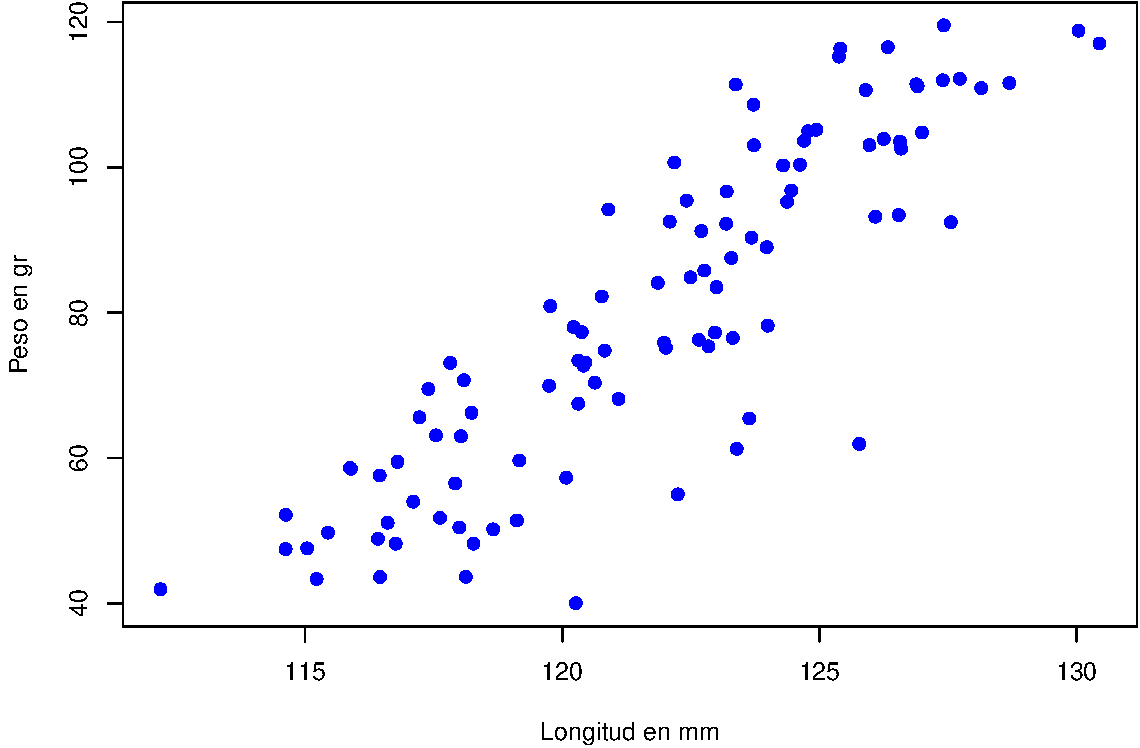
\includegraphics{tema7_files/figure-latex/unnamed-chunk-2-1.pdf}

La cuestión de interés es si existe alguna asociación entre la
probabilidad de una lectura ESR superior a 20 mm / hr y los niveles de
las dos proteínas plasmáticas. Si no es así, la determinación de ESR no
sería útil para fines de diagnóstico.

Dado que la variable de respuesta es binaria, un modelo de regresión
múltiple no es adecuado para un análisis de regresión.

Podemos escribir \[
\mathbb{P}\mbox{r}(y_i=1)=\pi_i \qquad \mathbb{P}\mbox{r}(y_i=0)=1-\pi_i
\]

El modelo

\[
  \mbox{logit}(\pi) = \mbox{logit}\left(\frac{\pi}{1-\pi}\right) = \beta_0 + \beta_1x_1 + ... + \beta_p x_p
\]

El logit de una probabilidad es simplemente el log de las probabilidades
de la respuesta tomando el valor una transformación logit o de p:
\(logit(p) = \log(p/1-p)\). Propiedades

\begin{itemize}
\tightlist
\item
  Si \texttt{odds(y=1)\ =\ 1}, entonces \texttt{logit(p)\ =\ 0}.
\item
  Si \texttt{odds(y=1)\ \textless{}\ 1}, entonces
  \texttt{logit(p)\ \textless{}\ 0}.
\item
  Si \texttt{odds(y=1)\ \textgreater{}\ 1}, entonces
  \texttt{logit(p)\ \textgreater{}\ 0}.
\end{itemize}

Cuando la respuesta es una variable binaria (dicotómica), y \(x\) es
numérica, la regresión logística ajusta una curva logística a la
relación entre \(x\) y \(y\). Por lo tanto, la regresión logística es la
regresión lineal en la transformación logit de y, donde y es la
proporción (o probabilidad) de éxito en cada valor de \(x\). Sin
embargo, se evitar la tentación de hacer una regresión lineal, ya que ni
la normalidad ni la suposición de homoscedasticidad se satisfacen.

\begin{Shaded}
\begin{Highlighting}[]
\NormalTok{x <-}\StringTok{ }\KeywordTok{seq}\NormalTok{(-}\DecValTok{6}\NormalTok{,}\DecValTok{6}\NormalTok{,}\FloatTok{0.01}\NormalTok{)}
\NormalTok{logistic <-}\StringTok{ }\KeywordTok{exp}\NormalTok{(x)/(}\DecValTok{1}\NormalTok{+}\KeywordTok{exp}\NormalTok{(x))}
\KeywordTok{plot}\NormalTok{(x,logistic,}\DataTypeTok{t=}\StringTok{'l'}\NormalTok{,}\DataTypeTok{main=}\StringTok{"Logistic curve"}\NormalTok{,}\DataTypeTok{ylab=}\StringTok{"p"}\NormalTok{,}\DataTypeTok{xlab=}\StringTok{"log(p(1-p)"}\NormalTok{)}
\KeywordTok{abline}\NormalTok{(}\DataTypeTok{h=}\KeywordTok{c}\NormalTok{(}\DecValTok{0}\NormalTok{,}\FloatTok{0.5}\NormalTok{,}\DecValTok{1}\NormalTok{),}\DataTypeTok{v=}\DecValTok{0}\NormalTok{,}\DataTypeTok{col=}\StringTok{"grey"}\NormalTok{)}
\KeywordTok{points}\NormalTok{(}\DecValTok{0}\NormalTok{,}\FloatTok{0.5}\NormalTok{,}\DataTypeTok{pch=}\DecValTok{19}\NormalTok{,}\DataTypeTok{col=}\DecValTok{2}\NormalTok{)}
\end{Highlighting}
\end{Shaded}

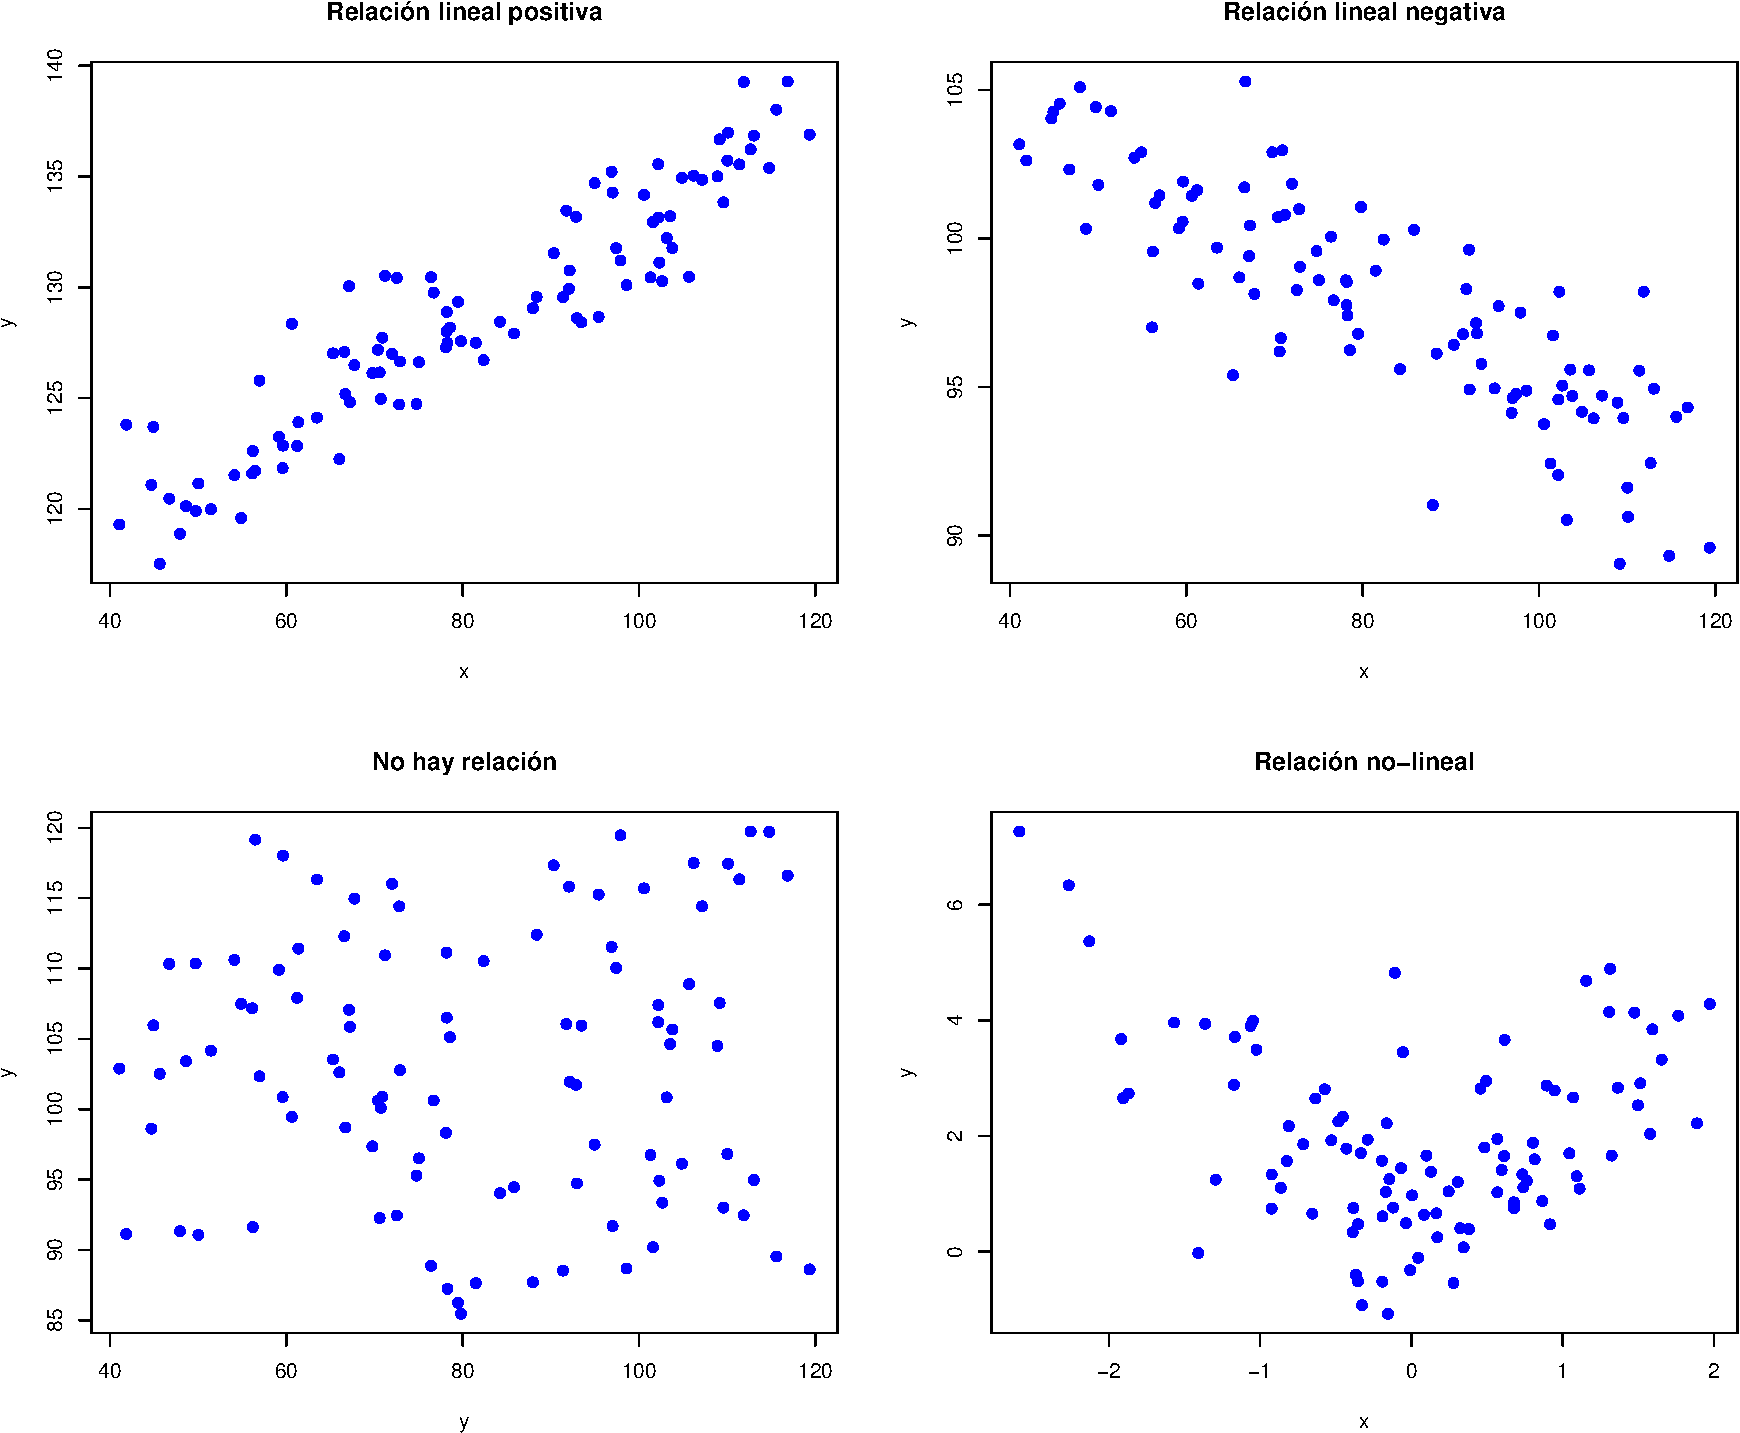
\includegraphics{tema7_files/figure-latex/unnamed-chunk-3-1.pdf}

La regresión logística en \texttt{R} se ajusta mediante la función
\texttt{glm}. En primer lugar, comenzamos con el modelo que incluye como
variable explicativa \texttt{fibrinogen}

\begin{Shaded}
\begin{Highlighting}[]
\NormalTok{plasma_glm_1 <-}\StringTok{ }\KeywordTok{glm}\NormalTok{(ESR ~}\StringTok{ }\NormalTok{fibrinogen, }\DataTypeTok{data =} \NormalTok{plasma,}\DataTypeTok{family =} \KeywordTok{binomial}\NormalTok{())}
\KeywordTok{summary}\NormalTok{(plasma_glm_1)}
\end{Highlighting}
\end{Shaded}

\begin{verbatim}
## 
## Call:
## glm(formula = ESR ~ fibrinogen, family = binomial(), data = plasma)
## 
## Deviance Residuals: 
##     Min       1Q   Median       3Q      Max  
## -0.9298  -0.5399  -0.4382  -0.3356   2.4794  
## 
## Coefficients:
##             Estimate Std. Error z value Pr(>|z|)  
## (Intercept)  -6.8451     2.7703  -2.471   0.0135 *
## fibrinogen    1.8271     0.9009   2.028   0.0425 *
## ---
## Signif. codes:  0 '***' 0.001 '**' 0.01 '*' 0.05 '.' 0.1 ' ' 1
## 
## (Dispersion parameter for binomial family taken to be 1)
## 
##     Null deviance: 30.885  on 31  degrees of freedom
## Residual deviance: 24.840  on 30  degrees of freedom
## AIC: 28.84
## 
## Number of Fisher Scoring iterations: 5
\end{verbatim}

Vemos que el coeficiente de regresión para \texttt{fibrinogen} es
significativo al nivel de \(5\%\). Un aumento de una unidad en esta
variable aumenta log-odds en favor de un valor ESR mayor que 20 por un
\(1,83\) estimado con \(95\%\) intervalo de confianza.

\begin{Shaded}
\begin{Highlighting}[]
\KeywordTok{confint}\NormalTok{(plasma_glm_1,}\DataTypeTok{parm=}\StringTok{"fibrinogen"}\NormalTok{)}
\end{Highlighting}
\end{Shaded}

\begin{verbatim}
## Waiting for profiling to be done...
\end{verbatim}

\begin{verbatim}
##     2.5 %    97.5 % 
## 0.3387619 3.9984921
\end{verbatim}

Estos valores son más útiles si se convierten a los valores
correspondientes para las probabilidades ellos mismos exponenciando la
estimación.

\begin{Shaded}
\begin{Highlighting}[]
\KeywordTok{exp}\NormalTok{(}\KeywordTok{coef}\NormalTok{(plasma_glm_1)[}\StringTok{"fibrinogen"}\NormalTok{])}
\end{Highlighting}
\end{Shaded}

\begin{verbatim}
## fibrinogen 
##   6.215715
\end{verbatim}

y el intervalo de confianza

\begin{Shaded}
\begin{Highlighting}[]
\KeywordTok{exp}\NormalTok{(}\KeywordTok{confint}\NormalTok{(plasma_glm_1, }\DataTypeTok{parm =} \StringTok{"fibrinogen"}\NormalTok{))}
\end{Highlighting}
\end{Shaded}

\begin{verbatim}
## Waiting for profiling to be done...
\end{verbatim}

\begin{verbatim}
##     2.5 %    97.5 % 
##  1.403209 54.515884
\end{verbatim}

El intervalo de confianza es muy amplio porque hay pocas observaciones
en general y muy pocos donde el valor ESR es mayor de 20. Sin embargo,
parece probable que el aumento de los valores de fibrinógeno conducir a
una mayor probabilidad de un valor ESR mayor de 20. Ahora podemos caber
un modelo de regresión logística que incluye ambas variables
explicativas utilizando el código.

\begin{Shaded}
\begin{Highlighting}[]
\NormalTok{plasma_glm_2 <-}\StringTok{ }\KeywordTok{glm}\NormalTok{(ESR ~}\StringTok{ }\NormalTok{fibrinogen +}\StringTok{ }\NormalTok{globulin, }\DataTypeTok{data =} \NormalTok{plasma,}\DataTypeTok{family =} \KeywordTok{binomial}\NormalTok{())}
\KeywordTok{summary}\NormalTok{(plasma_glm_2)}
\end{Highlighting}
\end{Shaded}

\begin{verbatim}
## 
## Call:
## glm(formula = ESR ~ fibrinogen + globulin, family = binomial(), 
##     data = plasma)
## 
## Deviance Residuals: 
##     Min       1Q   Median       3Q      Max  
## -0.9683  -0.6122  -0.3458  -0.2116   2.2636  
## 
## Coefficients:
##             Estimate Std. Error z value Pr(>|z|)  
## (Intercept) -12.7921     5.7963  -2.207   0.0273 *
## fibrinogen    1.9104     0.9710   1.967   0.0491 *
## globulin      0.1558     0.1195   1.303   0.1925  
## ---
## Signif. codes:  0 '***' 0.001 '**' 0.01 '*' 0.05 '.' 0.1 ' ' 1
## 
## (Dispersion parameter for binomial family taken to be 1)
## 
##     Null deviance: 30.885  on 31  degrees of freedom
## Residual deviance: 22.971  on 29  degrees of freedom
## AIC: 28.971
## 
## Number of Fisher Scoring iterations: 5
\end{verbatim}

El coeficiente de gamma globulina no es significativamente diferente de
cero.

Ambos modelos anidados se pueden comparar utilizando una prueba de razón
de verosimilitud con la función \texttt{anova}

\begin{Shaded}
\begin{Highlighting}[]
\KeywordTok{anova}\NormalTok{(plasma_glm_1, plasma_glm_2, }\DataTypeTok{test =} \StringTok{"Chisq"}\NormalTok{)}
\end{Highlighting}
\end{Shaded}

\begin{verbatim}
## Analysis of Deviance Table
## 
## Model 1: ESR ~ fibrinogen
## Model 2: ESR ~ fibrinogen + globulin
##   Resid. Df Resid. Dev Df Deviance Pr(>Chi)
## 1        30     24.840                     
## 2        29     22.971  1   1.8692   0.1716
\end{verbatim}

Por lo tanto, concluimos que la gamma globulina no está asociada con el
nivel de ESR.

La gráfica muestra claramente la probabilidad creciente de un valor de
\texttt{ESR} por encima de 20 (círculos más grandes) como los valores de
\texttt{fibrinogen} ya una en menor medida, un aumento de la gamma
globulina.

\begin{Shaded}
\begin{Highlighting}[]
\NormalTok{prob <-}\StringTok{ }\KeywordTok{predict}\NormalTok{(plasma_glm_2,}\DataTypeTok{type=}\StringTok{"response"}\NormalTok{)}
\KeywordTok{plot}\NormalTok{(globulin ~}\StringTok{ }\NormalTok{fibrinogen, }\DataTypeTok{data =} \NormalTok{plasma, }\DataTypeTok{xlim =} \KeywordTok{c}\NormalTok{(}\DecValTok{2}\NormalTok{, }\DecValTok{6}\NormalTok{),}\DataTypeTok{ylim =} \KeywordTok{c}\NormalTok{(}\DecValTok{25}\NormalTok{, }\DecValTok{55}\NormalTok{), }\DataTypeTok{pch =} \StringTok{"."}\NormalTok{)}
\KeywordTok{symbols}\NormalTok{(plasma$fibrinogen, plasma$globulin, }\DataTypeTok{circles =} \NormalTok{prob,}\DataTypeTok{add =} \OtherTok{TRUE}\NormalTok{)}
\end{Highlighting}
\end{Shaded}

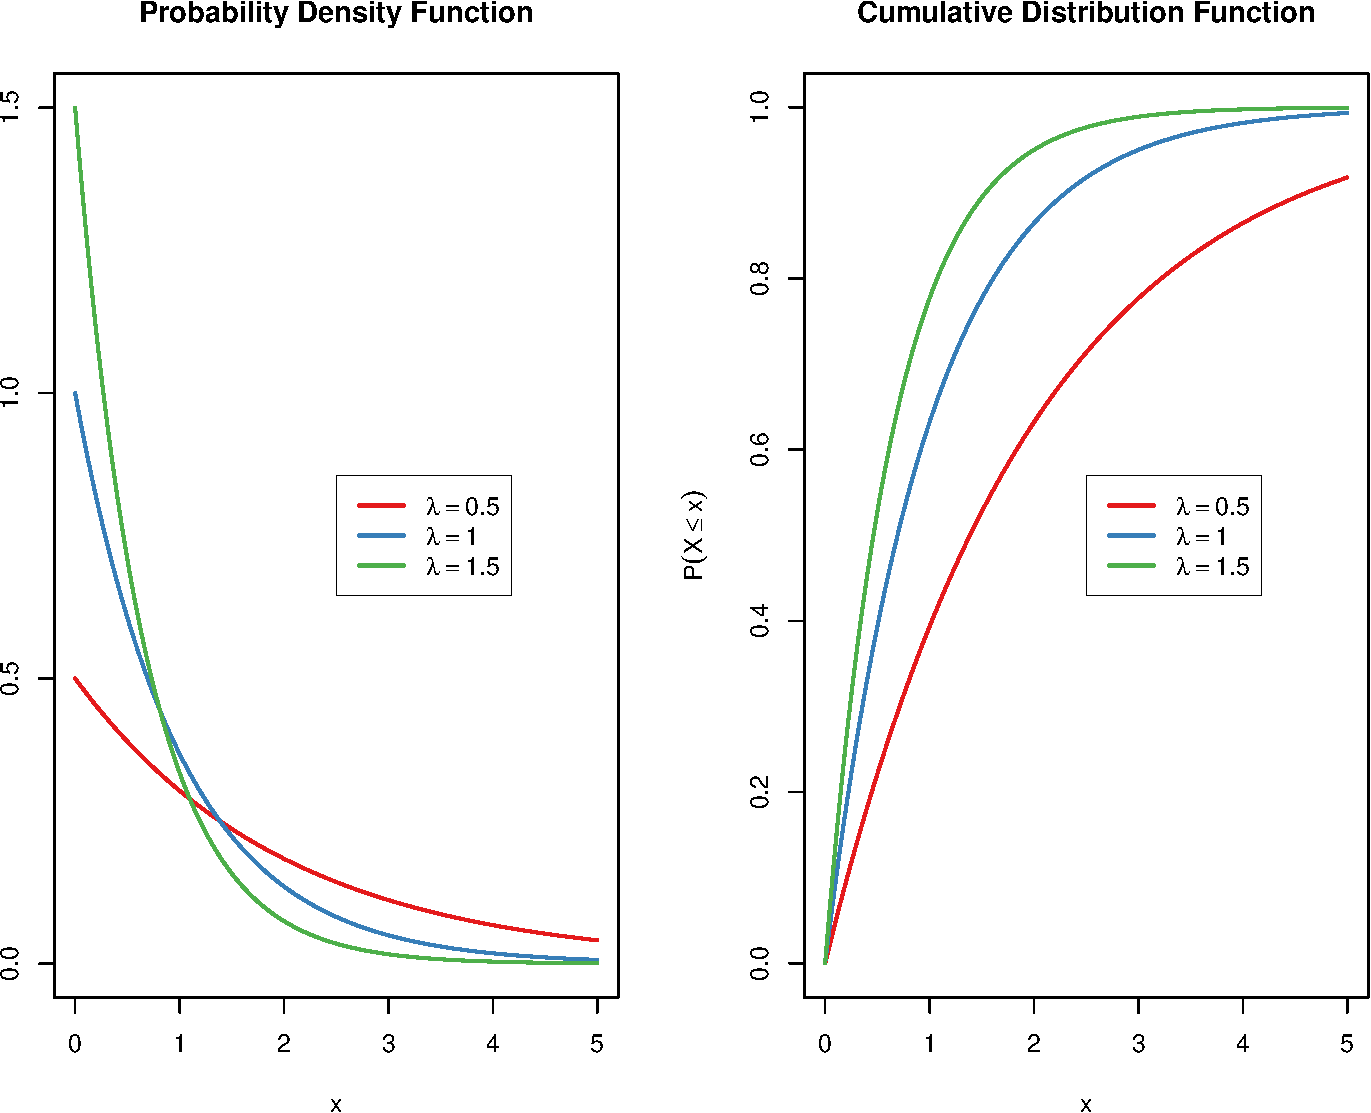
\includegraphics{tema7_files/figure-latex/unnamed-chunk-10-1.pdf}

\subsection{Casos de Estudio con la Regresión
Logística}\label{casos-de-estudio-con-la-regresion-logistica}

\textbf{Ejemplo:}

Supongamos el fichero de datos \texttt{adult.csv} disponible
\href{data/adult.csv}{aquí}

Vamos a tratar de predecir la variable respuesta \texttt{ABOVE50k}
(sueldo \textgreater{}50k) a través de una regresión logistica en base a
variables explicativas demográficas.

\begin{Shaded}
\begin{Highlighting}[]
\NormalTok{inputData <-}\StringTok{ }\KeywordTok{read.csv}\NormalTok{(}\StringTok{"http://idaejin.github.io/bcam-courses/R/datahack/Modulo1/data/adult.csv"}\NormalTok{)}
\end{Highlighting}
\end{Shaded}

\subsection{Sesgo de clase}\label{sesgo-de-clase}

Idealmente, la proporción de eventos y no eventos en la variable \(Y\)
debe ser aproximadamente la misma. Por lo tanto, primero vamos a
comprobar la proporción de clases en la variable dependiente
\texttt{ABOVE50K}.

Claramente, hay un \emph{sesgo de clase}, una condición observada cuando
la proporción de eventos es mucho menor que la proporción de no-eventos.
Por lo tanto, debemos muestrear las observaciones en proporciones
aproximadamente iguales para obtener mejores modelos.

\begin{Shaded}
\begin{Highlighting}[]
\KeywordTok{table}\NormalTok{(inputData$ABOVE50K)}
\end{Highlighting}
\end{Shaded}

\begin{verbatim}
## 
##     0     1 
## 24720  7841
\end{verbatim}

\subsection{Crear muestra de entrenamiento y de validación (o
test)}\label{crear-muestra-de-entrenamiento-y-de-validacion-o-test}

Una forma de abordar el problema del sesgo de clase es dibujar los 0 y 1
para el trainingData (muestra de desarrollo) en proporciones iguales. Al
hacerlo, pondremos el resto del inputData no incluido en el
entrenamiento en testData (muestra de validación). Como resultado, el
tamaño de la muestra de desarrollo será menor que la validación, lo que
está bien, porque, hay un gran número de observaciones (\textgreater{}
10K).

\begin{Shaded}
\begin{Highlighting}[]
\NormalTok{logitMod <-}\StringTok{ }\KeywordTok{glm}\NormalTok{(ABOVE50K ~}\StringTok{ }\NormalTok{RELATIONSHIP +}\StringTok{ }\NormalTok{AGE +}\StringTok{ }\NormalTok{CAPITALGAIN }
                \NormalTok{+}\StringTok{ }\NormalTok{OCCUPATION +}\StringTok{ }\NormalTok{EDUCATIONNUM, }\DataTypeTok{data=}\NormalTok{trainingData, }
                \DataTypeTok{family=}\KeywordTok{binomial}\NormalTok{(}\DataTypeTok{link=}\StringTok{"logit"}\NormalTok{))}
\end{Highlighting}
\end{Shaded}

\begin{verbatim}
## Warning: glm.fit: fitted probabilities numerically 0 or 1 occurred
\end{verbatim}

\begin{Shaded}
\begin{Highlighting}[]
\NormalTok{predicted <-}\StringTok{ }\KeywordTok{plogis}\NormalTok{(}\KeywordTok{predict}\NormalTok{(logitMod, testData))  }\CommentTok{# predicted scores or}
\CommentTok{# or}
\CommentTok{# predicted <- predict(logitMod, testData,type="response")  # predicted scores}
\end{Highlighting}
\end{Shaded}

Cuando usamos la función \texttt{predict()} en este modelo, se predice
el \texttt{log(odds)} de la variable \(Y\) (\(log(\frac{1}{1-p})\)).
Esto no es lo que queremos en última instancia porque, los valores
predichos pueden no estar dentro del rango 0 y 1 como se esperaba. Por
lo tanto, para convertirlo en puntajes de probabilidad de predicción que
están enlazados entre 0 y 1, usamos el \texttt{plogis()} o
\emph{type=``response''} como argumento de \texttt{predict()}.

\subsection{Decidir el límite óptimo de probabilidad de predicción para
el
modelo}\label{decidir-el-limite-optimo-de-probabilidad-de-prediccion-para-el-modelo}

La puntuación de probabilidad de predicción de corte por defecto es
\texttt{0,5} o la proporción de 1 y 0 en los datos de entrenamiento.
Pero a veces, afinar el límite de probabilidad puede mejorar la
precisión tanto en el desarrollo como en las muestras de validación. La
función del paquete \texttt{InformationValue} llamada
\texttt{optimalCutoff} proporciona maneras de encontrar el punto de
corte óptimo para mejorar la predicción de 1's, 0's, tanto 1 como 0's y
o reducir el error de clasificación errónea.

\begin{Shaded}
\begin{Highlighting}[]
\KeywordTok{library}\NormalTok{(InformationValue)}
\NormalTok{optCutOff <-}\StringTok{ }\KeywordTok{optimalCutoff}\NormalTok{(testData$ABOVE50K, predicted)[}\DecValTok{1}\NormalTok{]}
\NormalTok{optCutOff}
\end{Highlighting}
\end{Shaded}

\begin{verbatim}
## [1] 0.89
\end{verbatim}

\subsection{Error de clasificación
errónea}\label{error-de-clasificacion-erronea}

El error de clasificación errónea es el porcentaje de desajuste de los
valores reales predichos, independientemente de los 1 o los 0. Cuanto
menor sea el error de clasificación errónea, mejor será su modelo.

\begin{Shaded}
\begin{Highlighting}[]
\KeywordTok{misClassError}\NormalTok{(testData$ABOVE50K, predicted, }\DataTypeTok{threshold =} \NormalTok{optCutOff)}
\end{Highlighting}
\end{Shaded}

\begin{verbatim}
## [1] 0.0892
\end{verbatim}

\subsection{Curva ROC}\label{curva-roc}

La curva ROC (Receiver Operating Characteristics) es una representación
gráfica de la sensibilidad frente a la especificidad para un sistema
clasificador binario según se varía el umbral de discriminación.

Otra interpretación de este gráfico es la representación de la razón o
ratio de verdaderos positivos (VPR = Razón de Verdaderos Positivos)
frente a la razón o ratio de falsos positivos (FPR = Razón de Falsos
Positivos) también según se varía el umbral de discriminación (valor a
partir del cual decidimos que un caso es un positivo).

Proporciona herramientas para seleccionar los modelos posiblemente
óptimos y descartar modelos subóptimos independientemente de (y antes de
especificar) el coste de la distribución de las dos clases sobre las que
se decide.

\begin{itemize}
\item
  Verdaderos Positivos (VP) o también éxitos
\item
  Verdaderos Negativos (VN) o también rechazos correctos
\item
  Falsos Positivos (FP) o también falsas alarmas o Error tipo I
\item
  Falsos Negativos (FN) o también, Error de tipo II
\item
  Sensibilidad o Razón de Verdaderos Positivos (VPR) o también razón de
  éxitos y, recuerdo en recuperación de información,
\end{itemize}

\[
VPR=VP/P=VP/(VP+FN)
\]

\begin{itemize}
\tightlist
\item
  Especificidad o Razón de Verdaderos Negativos
\end{itemize}

\[
\mbox{ESPECIFICIDAD}=VN/N=VN/(FP+VN)=1-FPR
\]

\begin{Shaded}
\begin{Highlighting}[]
\KeywordTok{plotROC}\NormalTok{(testData$ABOVE50K, predicted)}
\end{Highlighting}
\end{Shaded}

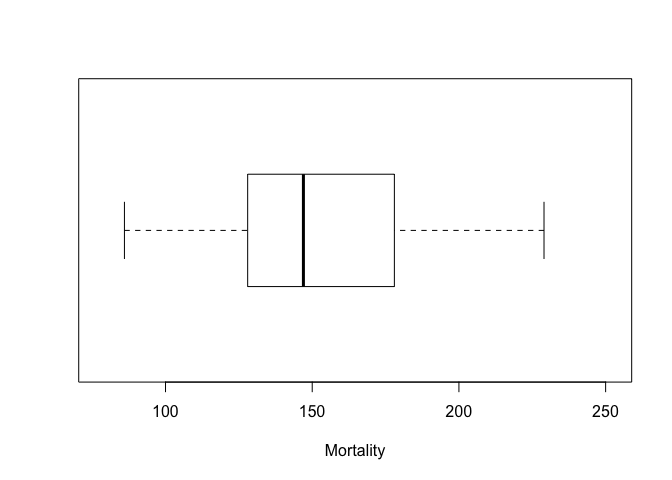
\includegraphics{tema7_files/figure-latex/unnamed-chunk-17-1.pdf}

\subsubsection{German credit Data}\label{german-credit-data}

\begin{Shaded}
\begin{Highlighting}[]
\NormalTok{data <-}\StringTok{ }\KeywordTok{read.table}\NormalTok{(}\StringTok{"http://ftp.ics.uci.edu/pub/machine-learning-databases/statlog/german/german.data"}\NormalTok{, }\DataTypeTok{header =} \OtherTok{FALSE}\NormalTok{)}

\KeywordTok{colnames}\NormalTok{(data)<-}\KeywordTok{c}\NormalTok{(}\StringTok{"account.status"}\NormalTok{,}\StringTok{"months"}\NormalTok{,}
                \StringTok{"credit.history"}\NormalTok{,}\StringTok{"purpose"}\NormalTok{,}\StringTok{"credit.amount"}\NormalTok{,}
                \StringTok{"savings"}\NormalTok{,}\StringTok{"employment"}\NormalTok{,}\StringTok{"installment.rate"}\NormalTok{,}\StringTok{"personal.status"}\NormalTok{,}
                \StringTok{"guarantors"}\NormalTok{,}\StringTok{"residence"}\NormalTok{,}\StringTok{"property"}\NormalTok{,}\StringTok{"age"}\NormalTok{,}\StringTok{"other.installments"}\NormalTok{,}
                \StringTok{"housing"}\NormalTok{,}\StringTok{"credit.cards"}\NormalTok{,}\StringTok{"job"}\NormalTok{,}\StringTok{"dependents"}\NormalTok{,}\StringTok{"phone"}\NormalTok{,}\StringTok{"foreign.worker"}\NormalTok{,}\StringTok{"credit.rating"}\NormalTok{)}

\KeywordTok{head}\NormalTok{(data)}
\end{Highlighting}
\end{Shaded}

\begin{verbatim}
##   account.status months credit.history purpose credit.amount savings
## 1            A11      6            A34     A43          1169     A65
## 2            A12     48            A32     A43          5951     A61
## 3            A14     12            A34     A46          2096     A61
## 4            A11     42            A32     A42          7882     A61
## 5            A11     24            A33     A40          4870     A61
## 6            A14     36            A32     A46          9055     A65
##   employment installment.rate personal.status guarantors residence
## 1        A75                4             A93       A101         4
## 2        A73                2             A92       A101         2
## 3        A74                2             A93       A101         3
## 4        A74                2             A93       A103         4
## 5        A73                3             A93       A101         4
## 6        A73                2             A93       A101         4
##   property age other.installments housing credit.cards  job dependents
## 1     A121  67               A143    A152            2 A173          1
## 2     A121  22               A143    A152            1 A173          1
## 3     A121  49               A143    A152            1 A172          2
## 4     A122  45               A143    A153            1 A173          2
## 5     A124  53               A143    A153            2 A173          2
## 6     A124  35               A143    A153            1 A172          2
##   phone foreign.worker credit.rating
## 1  A192           A201             1
## 2  A191           A201             2
## 3  A191           A201             1
## 4  A191           A201             1
## 5  A191           A201             2
## 6  A192           A201             1
\end{verbatim}

\begin{Shaded}
\begin{Highlighting}[]
\KeywordTok{levels}\NormalTok{(data$account.status) <-}\StringTok{ }\KeywordTok{c}\NormalTok{(}\StringTok{"<0DM"}\NormalTok{,}\StringTok{"<200DM"}\NormalTok{,}\StringTok{">200DM"}\NormalTok{,}\StringTok{"NoStatus"}\NormalTok{)}
\KeywordTok{levels}\NormalTok{(data$credit.history) <-}\StringTok{ }\KeywordTok{c}\NormalTok{(}\StringTok{"No"}\NormalTok{,}\StringTok{"Allpaid"}\NormalTok{,}\StringTok{"Allpaidtillnow"}\NormalTok{,}\StringTok{"Delayinpaying"}\NormalTok{,}\StringTok{"Critical"}\NormalTok{)}
\KeywordTok{levels}\NormalTok{(data$purpose) <-}\StringTok{ }\KeywordTok{c}\NormalTok{(}\StringTok{"car(new)"}\NormalTok{,}\StringTok{"car(used)"}\NormalTok{,}\StringTok{"furniture/equipment"}\NormalTok{,}\StringTok{"radio/television"}\NormalTok{,}\StringTok{"domesticappliances"}\NormalTok{,}
\StringTok{"repairs"}\NormalTok{,}\StringTok{"education"}\NormalTok{,}\StringTok{"vacation-doesnotexist?"}\NormalTok{,}\StringTok{"retraining"}\NormalTok{,}\StringTok{"business"}\NormalTok{,}\StringTok{"others"}\NormalTok{)}
\end{Highlighting}
\end{Shaded}

Vamos a dividir el conjunto de datos en 0.7: 0.3 para el entrenamiento y
la prueba del modelo. Para la regresión logística, también necesitamos
transformar el marco de datos con factores en la matriz con valor
biométrico.

\begin{Shaded}
\begin{Highlighting}[]
\NormalTok{mat1 <-}\StringTok{ }\KeywordTok{model.matrix}\NormalTok{(credit.rating ~}\StringTok{ }\NormalTok{. , }\DataTypeTok{data =} \NormalTok{data)}
\NormalTok{n<-}\StringTok{ }\KeywordTok{dim}\NormalTok{(data)[}\DecValTok{1}\NormalTok{]}

\KeywordTok{set.seed}\NormalTok{(}\DecValTok{1234}\NormalTok{)}
\NormalTok{train<-}\StringTok{ }\KeywordTok{sample}\NormalTok{(}\DecValTok{1}\NormalTok{:n , }\FloatTok{0.7}\NormalTok{*n)}
\NormalTok{xtrain<-}\StringTok{ }\NormalTok{mat1[train,]}
\NormalTok{xtest<-}\StringTok{ }\NormalTok{mat1[-train,]}

\NormalTok{ytrain<-}\StringTok{ }\NormalTok{data$credit.rating[train]}
\NormalTok{ytrain <-}\StringTok{ }\KeywordTok{as.factor}\NormalTok{(ytrain}\DecValTok{-1}\NormalTok{) }\CommentTok{# convert to 0/1 factor}
 \NormalTok{ytest<-}\StringTok{ }\NormalTok{data$credit.rating[-train]}
\NormalTok{ytest  <-}\StringTok{ }\KeywordTok{as.factor}\NormalTok{(ytest}\DecValTok{-1}\NormalTok{) }\CommentTok{#  convert to 0/1 factor}
\end{Highlighting}
\end{Shaded}

Build the logistic Regression model

\begin{Shaded}
\begin{Highlighting}[]
\NormalTok{m1 <-}\StringTok{ }\KeywordTok{glm}\NormalTok{(credit.rating ~}\StringTok{ }\NormalTok{. , }\DataTypeTok{family =} \NormalTok{binomial, }\DataTypeTok{data=} \KeywordTok{data.frame}\NormalTok{(}\DataTypeTok{credit.rating=} \NormalTok{ytrain, xtrain))}
\end{Highlighting}
\end{Shaded}

Key Variables for the regression model.

\begin{Shaded}
\begin{Highlighting}[]
\NormalTok{sig.var<-}\StringTok{ }\KeywordTok{summary}\NormalTok{(m1)$coeff[-}\DecValTok{1}\NormalTok{,}\DecValTok{4}\NormalTok{] <}\FloatTok{0.01}
\KeywordTok{names}\NormalTok{(sig.var)[sig.var ==}\StringTok{ }\NormalTok{T]}
\end{Highlighting}
\end{Shaded}

\begin{verbatim}
## [1] "account.statusNoStatus"    "months"                   
## [3] "credit.historyCritical"    "purposecar.used."         
## [5] "purposeradio.television"   "purposedomesticappliances"
## [7] "savingsA64"                "savingsA65"               
## [9] "installment.rate"
\end{verbatim}

Predict outcome with Logistic Regression model, then use the test
dataset to evaluate the model.

\begin{Shaded}
\begin{Highlighting}[]
\NormalTok{pred1<-}\StringTok{ }\KeywordTok{predict.glm}\NormalTok{(m1,}\DataTypeTok{newdata =} \KeywordTok{data.frame}\NormalTok{(ytest,xtest), }\DataTypeTok{type=}\StringTok{"response"}\NormalTok{)}
\end{Highlighting}
\end{Shaded}

\begin{verbatim}
## Warning in predict.lm(object, newdata, se.fit, scale = 1, type =
## ifelse(type == : prediction from a rank-deficient fit may be misleading
\end{verbatim}

\begin{Shaded}
\begin{Highlighting}[]
\NormalTok{result1<-}\StringTok{ }\KeywordTok{table}\NormalTok{(ytest, }\KeywordTok{floor}\NormalTok{(pred1}\FloatTok{+1.5}\NormalTok{))}
\NormalTok{result1}
\end{Highlighting}
\end{Shaded}

\begin{verbatim}
##      
## ytest   1   2
##     0 176  25
##     1  51  48
\end{verbatim}

\begin{Shaded}
\begin{Highlighting}[]
\NormalTok{error1<-}\StringTok{ }\KeywordTok{sum}\NormalTok{(result1[}\DecValTok{1}\NormalTok{,}\DecValTok{2}\NormalTok{], result1[}\DecValTok{2}\NormalTok{,}\DecValTok{1}\NormalTok{])/}\KeywordTok{sum}\NormalTok{(result1)}
\NormalTok{error1}
\end{Highlighting}
\end{Shaded}

\begin{verbatim}
## [1] 0.2533333
\end{verbatim}

Curva ROC con el paquete \texttt{ROCR}

\begin{Shaded}
\begin{Highlighting}[]
\KeywordTok{library}\NormalTok{(ROCR)}
\end{Highlighting}
\end{Shaded}

\begin{verbatim}
## Loading required package: gplots
\end{verbatim}

\begin{verbatim}
## 
## Attaching package: 'gplots'
\end{verbatim}

\begin{verbatim}
## The following object is masked from 'package:stats':
## 
##     lowess
\end{verbatim}

\begin{Shaded}
\begin{Highlighting}[]
\NormalTok{pred =}\StringTok{ }\KeywordTok{prediction}\NormalTok{(pred1,ytest)}
\NormalTok{perf <-}\StringTok{ }\KeywordTok{performance}\NormalTok{(pred, }\StringTok{"tpr"}\NormalTok{, }\StringTok{"fpr"}\NormalTok{)}
\KeywordTok{plot}\NormalTok{(perf)}
\end{Highlighting}
\end{Shaded}

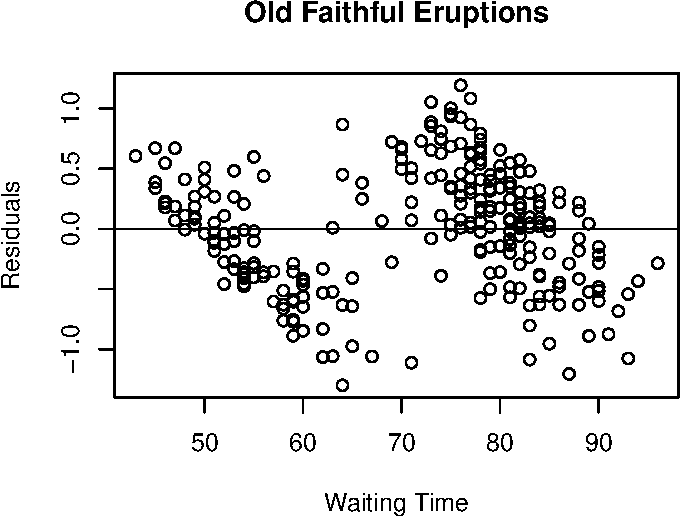
\includegraphics{tema7_files/figure-latex/unnamed-chunk-24-1.pdf}

\begin{Shaded}
\begin{Highlighting}[]
\NormalTok{AUCLog1=}\KeywordTok{performance}\NormalTok{(pred, }\DataTypeTok{measure =} \StringTok{"auc"}\NormalTok{)@y.values[[}\DecValTok{1}\NormalTok{]]}
\KeywordTok{cat}\NormalTok{(}\StringTok{"AUC: "}\NormalTok{,AUCLog1,}\StringTok{"n"}\NormalTok{)}
\end{Highlighting}
\end{Shaded}

\begin{verbatim}
## AUC:  0.7699382 n
\end{verbatim}

\section{Regresión de Poisson}\label{regresion-de-poisson}

En la regresión de Poisson la variable respuesta/resultado \(Y\) es un
conteo. Pero también podemos tener \(Y/t\), la tasa (o incidencia) como
la variable de respuesta, donde \(t\) es un intervalo que representa el
tiempo, el espacio o algún otro agrupamiento.

\textbf{Variables explicativas:}

\begin{itemize}
\item
  Las variables explicativas, \(X = (X_1, X_2, ... X_k)\), pueden ser
  continuas o una combinación de variables continuas y categóricas.
\item
  Las variables explicativas, \(X = (X_1, X_2, ... X_k)\), pueden ser
  TODAS categóricas. Entonces los conteos se representan en una tabla de
  contingencia, y la convención es llamar a tal modelo modelo
  log-lineal.
\item
  Si \(Y/t\) es la variable de interés, entonces, incluso con todos los
  predictores categóricos, el modelo de regresión será conocido como
  regresión de Poisson, no un modelo log-lineal.
\end{itemize}

En la regresión de Poisson, los datos siguen una distribución de
\{Poisson\} distribution, i.e. \(y \sim \mathcal{P}\mbox{ois}(\mu)\). En
la regresión se utiliza la transformación del logaritmo

\[
\log(\mu)=\beta_0+\beta_1x_1
\] Por tanto, en teoría \(\mathbb{E}[y] = \mathbb{V}\mbox{ar}[y] = \mu\)

Por simplicidad, con una sola variable explicativa, escribimos:
\(\log(\mu)=\alpha + \beta_x\), que es equivalente a
\(\mu=exp(\alpha+\beta_x)=exp(\alpha)exp(\beta_x)\).

\textbf{Interpretación de las estimaciones de parámetros:}

\begin{itemize}
\item
  \(exp(\alpha) =\) es el efecto sobre la media de \(Y\), es decir
  \(\mu\), cuando \(X = 0\)
\item
  \(exp(\beta) =\) para cada unidad adicional de \(X\), la variable
  predictora tiene un efecto multiplicativo de \(exp(\beta)\) sobre la
  media de \(Y\), esto es \(\mu\)

  \begin{itemize}
  \item
    Si \(\beta = 0\), entonces \(exp(\beta) = 1\), y el conteo esperado,
    \(\mu = E(y) = exp(\alpha)\), por tanto \(Y\) y \(X\) no están
    relacionadas.
  \item
    Si \(\beta > 0\), entonces \(exp(\beta) > 1\), y el conteo esperado
    \(\mu = E(y)\) es \(exp(\beta)\) veces más grande cuando \(X = 0\)
  \item
    Si \(\beta < 0\), entonces \(exp(\beta) < 1\), y el conteo esperado
    \(\mu = E(y)\) es \(exp(\beta)\) veces más pequeño cuando \(X = 0\)
  \end{itemize}
\end{itemize}

\textbf{Ejemplo}

\begin{verbatim}
 horas   fisuras
 400        0
 1000      212
 1400       66
 1800      511
 2200      150
 2600      351
 3000      378
 3400       78
 3800      748
 4200      840
 4600      756
\end{verbatim}

\begin{Shaded}
\begin{Highlighting}[]
\NormalTok{turbinas <-}\StringTok{ }\KeywordTok{read.table}\NormalTok{(}\StringTok{"https://idaejin.github.io/bcam-courses/R/datahack/Modulo1/data/fisuras.txt"}\NormalTok{,}\DataTypeTok{header =} \OtherTok{TRUE}\NormalTok{)}
\KeywordTok{plot}\NormalTok{(turbinas,}\DataTypeTok{type=}\StringTok{"h"}\NormalTok{); }\KeywordTok{points}\NormalTok{(turbinas,}\DataTypeTok{cex=}\NormalTok{.}\DecValTok{6}\NormalTok{,}\DataTypeTok{pch=}\DecValTok{19}\NormalTok{)}
\end{Highlighting}
\end{Shaded}

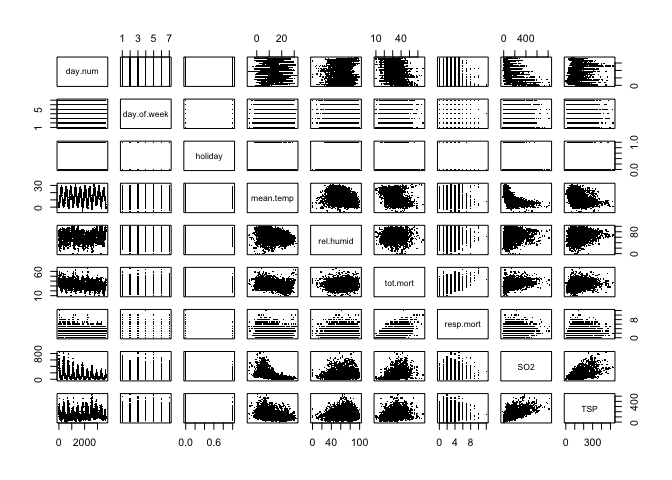
\includegraphics{tema7_files/figure-latex/unnamed-chunk-25-1.pdf}

\begin{Shaded}
\begin{Highlighting}[]
\NormalTok{ex2<-}\StringTok{ }\KeywordTok{lm}\NormalTok{(fisuras~horas,}\DataTypeTok{data=}\NormalTok{turbinas)}
\end{Highlighting}
\end{Shaded}

valores ajustados

\begin{Shaded}
\begin{Highlighting}[]
\NormalTok{ex2$fitted}
\end{Highlighting}
\end{Shaded}

\begin{Shaded}
\begin{Highlighting}[]
\KeywordTok{plot}\NormalTok{(turbinas,}\DataTypeTok{type=}\StringTok{"h"}\NormalTok{); }\KeywordTok{points}\NormalTok{(turbinas,}\DataTypeTok{cex=}\NormalTok{.}\DecValTok{6}\NormalTok{,}\DataTypeTok{pch=}\DecValTok{19}\NormalTok{)}
\KeywordTok{abline}\NormalTok{(ex2,}\DataTypeTok{col=}\DecValTok{2}\NormalTok{,}\DataTypeTok{lwd=}\DecValTok{2}\NormalTok{)}
\end{Highlighting}
\end{Shaded}

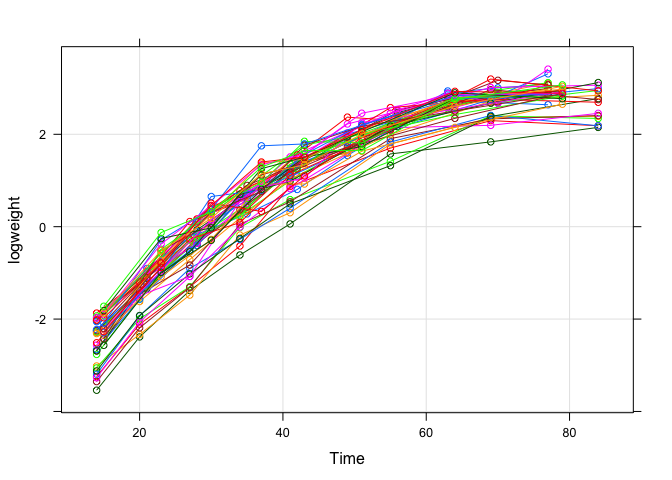
\includegraphics{tema7_files/figure-latex/unnamed-chunk-27-1.pdf}

\textbf{\texttt{family="poisson"}}

\begin{Shaded}
\begin{Highlighting}[]
\NormalTok{ex3 <-}\StringTok{ }\KeywordTok{glm}\NormalTok{(fisuras ~}\StringTok{ }\NormalTok{horas,}\DataTypeTok{data=}\NormalTok{turbinas, }\DataTypeTok{family =} \StringTok{"poisson"}\NormalTok{)}
\KeywordTok{plot}\NormalTok{(turbinas,}\DataTypeTok{type=}\StringTok{"h"}\NormalTok{); }\KeywordTok{points}\NormalTok{(turbinas,}\DataTypeTok{cex=}\NormalTok{.}\DecValTok{6}\NormalTok{,}\DataTypeTok{pch=}\DecValTok{19}\NormalTok{)}
\KeywordTok{lines}\NormalTok{(turbinas$horas,}\KeywordTok{fitted}\NormalTok{(ex3,}\DataTypeTok{type=}\StringTok{"response"}\NormalTok{),}\DataTypeTok{col=}\DecValTok{4}\NormalTok{,}\DataTypeTok{lwd=}\DecValTok{2}\NormalTok{)}
\end{Highlighting}
\end{Shaded}

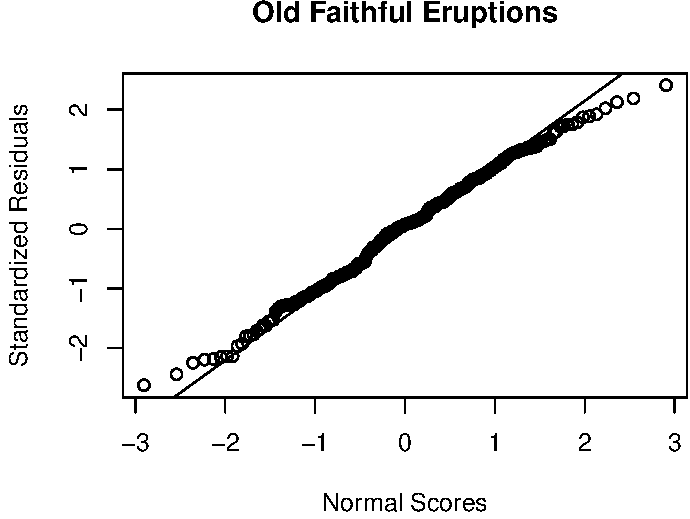
\includegraphics{tema7_files/figure-latex/unnamed-chunk-28-1.pdf}

\subsection{Regresión de Poisson para
tasas}\label{regresion-de-poisson-para-tasas}

Logaritmo de la tasa: \(\log(Y/t)\)

El modelo de regresión para la tasa esperada de ocurrencia es: \[
\log(\mu/t)= \alpha + \beta x
\]

que se puede reescribir como

\begin{eqnarray*}
\log(\mu)-\log(t) &= & \alpha +  \beta x \\
\log(\mu) & =& \alpha + \beta x + \log(t) \\
\end{eqnarray*}

El termino \(\log(t)\) se denomina \emph{offset}. Es un término de
ajuste y un grupo de observaciones puede tener el mismo \texttt{offset}
o cada individuo puede tener un valor diferente de \(t\). \(\log(t)\) es
una observación y cambiará el valor de los recuentos estimados:

\[
\mu =exp(\alpha+\beta x+\log(t))=(t)exp(\alpha)exp(\beta_x)
\]

Esto significa que el conte medio es proporcional a \(t\).

\textbf{Ejemplo:}

Los datos \texttt{credit.data} son una muestra de sujetos seleccionados
aleatoriamente para un estudio italiano sobre la relación entre ingresos
y si se posee una tarjeta de crédito de viaje (como American Express o
Diner's Club). En cada nivel de ingresos anuales en millones de liras
(la moneda en Italia antes del euro), el cuadro indica el número de
sujetos que se tomaron muestras y el número de estos sujetos que poseen
al menos una tarjeta de crédito de viaje.

Este ejemplo tiene información sobre los individuos agrupados por sus
ingresos, el número de individuos (casos) dentro de ese grupo de
ingresos y el número de tarjetas de crédito.

\begin{Shaded}
\begin{Highlighting}[]
\NormalTok{credit.card <-}\StringTok{ }\KeywordTok{read.table}\NormalTok{(}\StringTok{"https://idaejin.github.io/bcam-courses/R/datahack/Modulo1/data/creditcard.txt"}\NormalTok{)}
\KeywordTok{names}\NormalTok{(credit.card) <-}\StringTok{ }\KeywordTok{c}\NormalTok{(}\StringTok{"Income"}\NormalTok{,}\StringTok{"NumberCases"}\NormalTok{,}\StringTok{"CreditCards"}\NormalTok{)}

\CommentTok{# creamos la variable lcases como offset}
\NormalTok{lcases <-}\StringTok{ }\KeywordTok{log}\NormalTok{(credit.card[,}\DecValTok{2}\NormalTok{])}

\NormalTok{data <-}\StringTok{ }\KeywordTok{cbind}\NormalTok{(credit.card,lcases)}
\end{Highlighting}
\end{Shaded}

\texttt{offset} sirve para normalizar los valores de la celda celda
ajustada por algún espacio, agrupación o intervalo de tiempo con el fin
de modelar las tasas.

variable serves to normalize the fitted cell means per some space,
grouping or time interval in order to model the rates

\begin{Shaded}
\begin{Highlighting}[]
\NormalTok{poisson.mod <-}\StringTok{ }\KeywordTok{glm}\NormalTok{(CreditCards~Income+}\KeywordTok{offset}\NormalTok{(lcases),}\DataTypeTok{family=}\NormalTok{poisson, data)}
\KeywordTok{summary}\NormalTok{(poisson.mod)}
\end{Highlighting}
\end{Shaded}

\begin{verbatim}
## 
## Call:
## glm(formula = CreditCards ~ Income + offset(lcases), family = poisson, 
##     data = data)
## 
## Deviance Residuals: 
##     Min       1Q   Median       3Q      Max  
## -1.6907  -0.9329  -0.5675   0.2186   2.1681  
## 
## Coefficients:
##              Estimate Std. Error z value Pr(>|z|)    
## (Intercept) -2.386586   0.399655  -5.972 2.35e-09 ***
## Income       0.020758   0.005165   4.019 5.84e-05 ***
## ---
## Signif. codes:  0 '***' 0.001 '**' 0.01 '*' 0.05 '.' 0.1 ' ' 1
## 
## (Dispersion parameter for poisson family taken to be 1)
## 
##     Null deviance: 42.078  on 30  degrees of freedom
## Residual deviance: 28.465  on 29  degrees of freedom
## AIC: 67.604
## 
## Number of Fisher Scoring iterations: 5
\end{verbatim}

El modelo es: \[
log(\mu/t) = -2.3866 + 0.0208 × Income
\] donde \(log(t)\) = casos.

¿Cuál es la tasa promedio estimada de incidencia, es decir, el uso de
tarjetas de crédito dado el ingreso?

También podemos obtener el número predicho/ajustado/ esperado de
tarjetas de crédito basado en el modelo ajustado.

\begin{Shaded}
\begin{Highlighting}[]
\KeywordTok{fitted}\NormalTok{(poisson.mod)}
\end{Highlighting}
\end{Shaded}

\begin{verbatim}
##         1         2         3         4         5         6         7 
## 0.1513140 0.1610364 0.8220707 0.5035881 1.5424521 0.8748915 1.4291875 
##         8         9        10        11        12        13        14 
## 0.1823956 1.3035488 0.1901272 0.6070306 0.4131753 1.0546039 0.4306896 
##        15        16        17        18        19        20        21 
## 0.4397232 0.2339885 0.2490230 0.2542462 2.5957899 0.2705824 0.3128994 
##        22        23        24        25        26        27        28 
## 1.5973118 2.1264053 1.1315170 1.9658025 0.4739200 0.4838604 0.5257510 
##        29        30        31 
## 0.6470388 6.6599658 1.3660636
\end{verbatim}

Así, en el grupo de seis personas que ganan unos 65 millones de liras,
el número esperado en el grupo con al menos una tarjeta de crédito de
viaje es 2.126, mientras que el número observado es de 6.

\begin{Shaded}
\begin{Highlighting}[]
\KeywordTok{predict}\NormalTok{(poisson.mod,}\KeywordTok{data.frame}\NormalTok{(}\DataTypeTok{lcases=}\KeywordTok{log}\NormalTok{(}\DecValTok{6}\NormalTok{),}\DataTypeTok{Income=}\DecValTok{65}\NormalTok{),}\DataTypeTok{type=}\StringTok{"response"}\NormalTok{)}
\end{Highlighting}
\end{Shaded}

\begin{verbatim}
##        1 
## 2.126405
\end{verbatim}

\(\hat{\mu}=2.1264053\).

Notese, que \texttt{lcases\ =\ log(t)\ =\ log(6)} para este caso
específico. La tasa esperada sería

\[
 \frac{\hat{\mu}}{t} \approx 0.3544
\]

\textbf{Desastre del transbordador Challenger}

El 7 de Enero de 1986, la noche antes del despegue del transbordador,
hubo una reunión en la que se discutio sobre la la temperatura mínima
predicha para del día siguiente, 31F, y el efecto de la misma sobre el
sello en las juntas de los O-rings. En la discusión utilizaron el
siguiente gráfico en el que se muestra la relación entre la temperatura
y el número de O-rings que sufrian problemas

\begin{Shaded}
\begin{Highlighting}[]
\NormalTok{challenger<-}\KeywordTok{read.table}\NormalTok{(}\StringTok{"http://idaejin.github.io/bcam-courses/R/datahack/Modulo1/data/challenger.csv"}\NormalTok{, }\DataTypeTok{header=}\OtherTok{TRUE}\NormalTok{, }\DataTypeTok{sep=}\StringTok{","}\NormalTok{)}
\NormalTok{m<-challenger[,}\DecValTok{1}\NormalTok{]}
\NormalTok{r<-challenger[,}\DecValTok{2}\NormalTok{]}
\NormalTok{temperature<-challenger[,}\DecValTok{3}\NormalTok{]}

\NormalTok{### plot all data}
\KeywordTok{plot}\NormalTok{(temperature, r,}\DataTypeTok{pch=}\DecValTok{19}\NormalTok{,}\DataTypeTok{cex=}\FloatTok{1.65}\NormalTok{,}\DataTypeTok{xlim=}\KeywordTok{c}\NormalTok{(}\DecValTok{50}\NormalTok{,}\DecValTok{85}\NormalTok{),}\DataTypeTok{ylim=}\KeywordTok{c}\NormalTok{(-}\FloatTok{0.05}\NormalTok{,}\FloatTok{2.5}\NormalTok{),}
     \DataTypeTok{xlab=}\StringTok{'Joint temperature / F'}\NormalTok{, }\DataTypeTok{ylab=}\StringTok{'No. of O-ring failures'}\NormalTok{,}\DataTypeTok{col=}\StringTok{"blue"}\NormalTok{)}
\end{Highlighting}
\end{Shaded}

\includegraphics{tema7_files/figure-latex/unnamed-chunk-33-1.pdf}

\begin{Shaded}
\begin{Highlighting}[]
\KeywordTok{par}\NormalTok{(}\DataTypeTok{xaxs=}\StringTok{"i"}\NormalTok{, }\DataTypeTok{yaxs=}\StringTok{"i"}\NormalTok{)}
\NormalTok{x.at <-}\StringTok{ }\KeywordTok{seq}\NormalTok{(}\DecValTok{20}\NormalTok{, }\DecValTok{80}\NormalTok{, }\DataTypeTok{by=}\DecValTok{5}\NormalTok{)}
\NormalTok{y.at <-}\StringTok{ }\KeywordTok{seq}\NormalTok{(}\DecValTok{0}\NormalTok{, }\DecValTok{6}\NormalTok{, }\DataTypeTok{by=}\DecValTok{1}\NormalTok{)}
\KeywordTok{plot}\NormalTok{(temperature, r, }\DataTypeTok{xlim=}\KeywordTok{range}\NormalTok{(x.at), }\DataTypeTok{ylim=}\KeywordTok{range}\NormalTok{(y.at),}
     \DataTypeTok{xlab=}\StringTok{'Joint temperature / F'}\NormalTok{, }\DataTypeTok{ylab=}\StringTok{'No. of O-ring failures'}\NormalTok{,}
     \DataTypeTok{pch=} \DecValTok{19}\NormalTok{,}\DataTypeTok{type=}\StringTok{"p"}\NormalTok{,}\DataTypeTok{axes=}\OtherTok{FALSE}\NormalTok{)}
\KeywordTok{axis}\NormalTok{(}\DecValTok{1}\NormalTok{, }\DataTypeTok{at=} \NormalTok{x.at, }\DataTypeTok{lwd.ticks =} \DecValTok{0}\NormalTok{)}
\KeywordTok{axis}\NormalTok{(}\DecValTok{2}\NormalTok{, }\DataTypeTok{at=} \NormalTok{y.at, }\DataTypeTok{lwd.ticks =} \DecValTok{0}\NormalTok{)}
\KeywordTok{abline}\NormalTok{(}\DataTypeTok{v=}\DecValTok{31}\NormalTok{, }\DataTypeTok{col=}\StringTok{'blue'}\NormalTok{)}
\KeywordTok{abline}\NormalTok{(}\DataTypeTok{h=}\DecValTok{6}\NormalTok{, }\DataTypeTok{col=}\StringTok{"black"}\NormalTok{)}
\KeywordTok{abline}\NormalTok{(}\DataTypeTok{v=}\DecValTok{80}\NormalTok{, }\DataTypeTok{col=}\StringTok{"black"}\NormalTok{)}
\end{Highlighting}
\end{Shaded}

\includegraphics{tema7_files/figure-latex/unnamed-chunk-33-2.pdf}

El primer error que cometieron, fue el no dibujar los casos en los que
no había incidentes, para saber cuál eran las temperaturas más
propicias. La decisición final fue permitir el despegue en el que
murieron 7 astronautas debido a la combustión de gas a través de un
O-ring. ng.

\begin{Shaded}
\begin{Highlighting}[]
\NormalTok{### original misleading plot!}
\KeywordTok{par}\NormalTok{(}\DataTypeTok{xaxs=}\StringTok{"i"}\NormalTok{, }\DataTypeTok{yaxs=}\StringTok{"i"}\NormalTok{)}
\NormalTok{x.at <-}\StringTok{ }\KeywordTok{seq}\NormalTok{(}\DecValTok{45}\NormalTok{, }\DecValTok{80}\NormalTok{, }\DataTypeTok{by=}\DecValTok{5}\NormalTok{)}
\NormalTok{y.at <-}\StringTok{ }\KeywordTok{seq}\NormalTok{(}\DecValTok{0}\NormalTok{, }\DecValTok{3}\NormalTok{, }\DataTypeTok{by=}\DecValTok{1}\NormalTok{)}
\NormalTok{failures <-}\StringTok{ }\KeywordTok{which}\NormalTok{(r!=}\DecValTok{0}\NormalTok{) ## selects failure cases}
\KeywordTok{plot}\NormalTok{(temperature[failures], r[failures],}\DataTypeTok{xlim =} \KeywordTok{range}\NormalTok{(x.at), }\DataTypeTok{ylim=} \KeywordTok{range}\NormalTok{(y.at),}
     \DataTypeTok{pch=} \DecValTok{19}\NormalTok{,}\DataTypeTok{type=} \StringTok{"p"}\NormalTok{, }\DataTypeTok{xlab=}\StringTok{'Calculated Joint Temperature F'}\NormalTok{,}
     \DataTypeTok{ylab=}\StringTok{'Number of Incidents'}\NormalTok{, }\DataTypeTok{axes=}\OtherTok{FALSE}\NormalTok{,}\DataTypeTok{col=}\StringTok{"blue"}\NormalTok{,}\DataTypeTok{cex=}\FloatTok{1.65}\NormalTok{)}
\KeywordTok{axis}\NormalTok{(}\DecValTok{1}\NormalTok{, }\DataTypeTok{at=} \NormalTok{x.at, }\DataTypeTok{lwd.ticks =} \NormalTok{-}\DecValTok{1}\NormalTok{)}
\KeywordTok{axis}\NormalTok{(}\DecValTok{2}\NormalTok{, }\DataTypeTok{at=} \NormalTok{y.at, }\DataTypeTok{lwd.ticks =} \NormalTok{-}\DecValTok{1}\NormalTok{)}
\KeywordTok{grid}\NormalTok{(}\DataTypeTok{ny=}\DecValTok{3}\NormalTok{, }\DataTypeTok{col=}\StringTok{"grey"}\NormalTok{, }\DataTypeTok{lty=}\StringTok{"solid"}\NormalTok{);}
\KeywordTok{abline}\NormalTok{(}\DataTypeTok{h=}\DecValTok{3}\NormalTok{, }\DataTypeTok{col=}\StringTok{"grey"}\NormalTok{)}
\end{Highlighting}
\end{Shaded}

\includegraphics{tema7_files/figure-latex/unnamed-chunk-34-1.pdf}

Regresión lineal?

\begin{Shaded}
\begin{Highlighting}[]
\NormalTok{### plot only launches with at least one failure and their fitted curve}
\NormalTok{failures <-}\StringTok{ }\KeywordTok{which}\NormalTok{(r!=}\DecValTok{0}\NormalTok{)}
\KeywordTok{par}\NormalTok{(}\DataTypeTok{xaxs=}\StringTok{"i"}\NormalTok{, }\DataTypeTok{yaxs=}\StringTok{"i"}\NormalTok{)}
\NormalTok{x.at <-}\StringTok{ }\KeywordTok{seq}\NormalTok{(}\DecValTok{20}\NormalTok{, }\DecValTok{80}\NormalTok{, }\DataTypeTok{by=}\DecValTok{5}\NormalTok{)}
\NormalTok{y.at <-}\StringTok{ }\KeywordTok{seq}\NormalTok{(}\DecValTok{0}\NormalTok{, }\DecValTok{3}\NormalTok{, }\DataTypeTok{by=}\DecValTok{1}\NormalTok{)}
\KeywordTok{plot}\NormalTok{(temperature[failures], r[failures], }\DataTypeTok{xlim=}\KeywordTok{range}\NormalTok{(x.at), }\DataTypeTok{ylim=}\KeywordTok{range}\NormalTok{(y.at),}
     \DataTypeTok{xlab=}\StringTok{'Joint temperature / F'}\NormalTok{, }\DataTypeTok{ylab=}\StringTok{'No. O-ring failures'}\NormalTok{,}\DataTypeTok{pch=} \DecValTok{19}\NormalTok{,}
     \DataTypeTok{type=} \StringTok{"p"}\NormalTok{, }\DataTypeTok{axes =} \NormalTok{F, }\DataTypeTok{cex=}\FloatTok{1.65}\NormalTok{,}\DataTypeTok{col=}\StringTok{"blue"}\NormalTok{)}
\KeywordTok{axis}\NormalTok{(}\DecValTok{1}\NormalTok{, }\DataTypeTok{at=} \NormalTok{x.at, }\DataTypeTok{lwd.ticks =} \DecValTok{0}\NormalTok{)}
\KeywordTok{axis}\NormalTok{(}\DecValTok{2}\NormalTok{, }\DataTypeTok{at=} \NormalTok{y.at, }\DataTypeTok{lwd.ticks =} \DecValTok{0}\NormalTok{)}
\KeywordTok{grid}\NormalTok{(}\DataTypeTok{ny=}\DecValTok{3}\NormalTok{, }\DataTypeTok{col=}\StringTok{"grey"}\NormalTok{, }\DataTypeTok{lty=}\StringTok{"solid"}\NormalTok{);}
\KeywordTok{abline}\NormalTok{(}\DataTypeTok{h=}\DecValTok{3}\NormalTok{, }\DataTypeTok{col=}\StringTok{"grey"}\NormalTok{)}
\NormalTok{testtemp <-}\StringTok{ }\KeywordTok{seq}\NormalTok{(}\DecValTok{10}\NormalTok{,}\DecValTok{100}\NormalTok{,}\DecValTok{1}\NormalTok{)}
\NormalTok{fit.lm <-}\StringTok{ }\KeywordTok{lm}\NormalTok{(r ~}\StringTok{ }\NormalTok{temperature, }\DataTypeTok{data=}\NormalTok{challenger, }\DataTypeTok{subset=}\KeywordTok{which}\NormalTok{(r!=}\DecValTok{0}\NormalTok{))}
\KeywordTok{lines}\NormalTok{(testtemp, }\KeywordTok{predict}\NormalTok{(fit.lm, }\KeywordTok{data.frame}\NormalTok{(}\DataTypeTok{temperature=}\NormalTok{testtemp)),}
      \DataTypeTok{col=}\StringTok{"red"}\NormalTok{,}\DataTypeTok{lwd=}\DecValTok{2}\NormalTok{)}
\end{Highlighting}
\end{Shaded}

\includegraphics{tema7_files/figure-latex/unnamed-chunk-35-1.pdf}

\begin{Shaded}
\begin{Highlighting}[]
\NormalTok{### plot all data}
\KeywordTok{par}\NormalTok{(}\DataTypeTok{xaxs=}\StringTok{"i"}\NormalTok{, }\DataTypeTok{yaxs=}\StringTok{"i"}\NormalTok{)}
\NormalTok{x.at <-}\StringTok{ }\KeywordTok{seq}\NormalTok{(}\DecValTok{20}\NormalTok{, }\DecValTok{80}\NormalTok{, }\DataTypeTok{by=}\DecValTok{5}\NormalTok{)}
\NormalTok{y.at <-}\StringTok{ }\KeywordTok{seq}\NormalTok{(}\DecValTok{0}\NormalTok{, }\DecValTok{10}\NormalTok{, }\DataTypeTok{by=}\DecValTok{1}\NormalTok{)}
\KeywordTok{plot}\NormalTok{(temperature, r, }\DataTypeTok{main =} \StringTok{"Scatterplot of all Data"}\NormalTok{, }\DataTypeTok{xlim=}\KeywordTok{range}\NormalTok{(x.at),}
     \DataTypeTok{ylim=}\KeywordTok{range}\NormalTok{(-}\FloatTok{0.1}\NormalTok{,y.at), }\DataTypeTok{xlab=}\StringTok{'Joint temperature / F'}\NormalTok{, }
     \DataTypeTok{ylab=}\StringTok{'No. of O-ring failures'}\NormalTok{,}\DataTypeTok{cex=}\FloatTok{1.65}\NormalTok{, }\DataTypeTok{col=}\StringTok{"blue"}\NormalTok{,}
     \DataTypeTok{pch=} \DecValTok{19}\NormalTok{,}\DataTypeTok{type=} \StringTok{"p"}\NormalTok{,}\DataTypeTok{axes=}\OtherTok{FALSE}\NormalTok{)}
\KeywordTok{axis}\NormalTok{(}\DecValTok{1}\NormalTok{, }\DataTypeTok{at=} \NormalTok{x.at, }\DataTypeTok{lwd.ticks =} \DecValTok{0}\NormalTok{)}
\KeywordTok{axis}\NormalTok{(}\DecValTok{2}\NormalTok{, }\DataTypeTok{at=} \NormalTok{y.at, }\DataTypeTok{lwd.ticks =} \DecValTok{0}\NormalTok{)}
\KeywordTok{abline}\NormalTok{(}\DataTypeTok{v=}\DecValTok{31}\NormalTok{, }\DataTypeTok{col=}\StringTok{'red'}\NormalTok{,}\DataTypeTok{lwd=}\DecValTok{3}\NormalTok{)}
\KeywordTok{abline}\NormalTok{(}\DataTypeTok{h=}\DecValTok{10}\NormalTok{, }\DataTypeTok{col=}\StringTok{"black"}\NormalTok{)}
\KeywordTok{abline}\NormalTok{(}\DataTypeTok{v=}\DecValTok{80}\NormalTok{, }\DataTypeTok{col=}\StringTok{"black"}\NormalTok{)}
\KeywordTok{legend}\NormalTok{(}\StringTok{"topright"}\NormalTok{, }\DataTypeTok{inset=}\NormalTok{.}\DecValTok{05}\NormalTok{,}\KeywordTok{c}\NormalTok{(}\StringTok{"Fitted Curve"}\NormalTok{,}\StringTok{"Temp at 31 F"}\NormalTok{),}
       \DataTypeTok{fill=}\KeywordTok{c}\NormalTok{(}\StringTok{"orange"}\NormalTok{, }\StringTok{"red"}\NormalTok{))}
\NormalTok{### Fit and plot a curve using all data}
\NormalTok{fit.glm <-}\StringTok{ }\KeywordTok{glm}\NormalTok{(}\KeywordTok{cbind}\NormalTok{(r,m-r) ~}\StringTok{ }\NormalTok{temperature, }\DataTypeTok{data=}\NormalTok{challenger, }\DataTypeTok{family=}\NormalTok{binomial)}
\CommentTok{# predict probability of failure of a single O-ring joint at the following temperature}
\NormalTok{testtemp <-}\StringTok{ }\KeywordTok{seq}\NormalTok{(}\DecValTok{10}\NormalTok{,}\DecValTok{100}\NormalTok{,}\DecValTok{1}\NormalTok{)}
\NormalTok{pred.glm <-}\StringTok{ }\KeywordTok{predict}\NormalTok{(fit.glm, }\KeywordTok{data.frame}\NormalTok{(}\DataTypeTok{temperature=}\NormalTok{testtemp), }
                    \DataTypeTok{type=}\StringTok{"response"}\NormalTok{,}\DataTypeTok{se.fit =} \OtherTok{TRUE} \NormalTok{)}
\KeywordTok{lines}\NormalTok{(testtemp, }\DecValTok{6}\NormalTok{*pred.glm$fit, }\DataTypeTok{col=}\StringTok{"orange"}\NormalTok{,}\DataTypeTok{lwd=}\DecValTok{3}\NormalTok{)}
\KeywordTok{lines}\NormalTok{(testtemp, }\DecValTok{6}\NormalTok{*pred.glm$fit}\FloatTok{-1.96}\NormalTok{*pred.glm$fit, }\DataTypeTok{col=}\StringTok{"orange"}\NormalTok{,}\DataTypeTok{lwd=}\DecValTok{3}\NormalTok{,}\DataTypeTok{lty=}\DecValTok{3}\NormalTok{)}
\KeywordTok{lines}\NormalTok{(testtemp, }\DecValTok{6}\NormalTok{*pred.glm$fit}\FloatTok{+1.96}\NormalTok{*pred.glm$fit, }\DataTypeTok{col=}\StringTok{"orange"}\NormalTok{,}\DataTypeTok{lwd=}\DecValTok{3}\NormalTok{,}\DataTypeTok{lty=}\DecValTok{3}\NormalTok{)}
\KeywordTok{points}\NormalTok{(temperature, r, }\DataTypeTok{main =} \StringTok{"Scatterplot of all Data"}\NormalTok{, }\DataTypeTok{xlim=}\KeywordTok{range}\NormalTok{(x.at),}
       \DataTypeTok{ylim=}\KeywordTok{range}\NormalTok{(-}\FloatTok{0.1}\NormalTok{,y.at), }\DataTypeTok{xlab=}\StringTok{'Joint temperature/F'}\NormalTok{,}
       \DataTypeTok{ylab=}\StringTok{'No. of O-ring failures'}\NormalTok{,}\DataTypeTok{cex=}\FloatTok{1.65}\NormalTok{, }\DataTypeTok{col=}\StringTok{"blue"}\NormalTok{,}\DataTypeTok{pch=} \DecValTok{19}\NormalTok{,}\DataTypeTok{type=} \StringTok{"p"}\NormalTok{)}
\end{Highlighting}
\end{Shaded}

\includegraphics{tema7_files/figure-latex/unnamed-chunk-36-1.pdf}

\end{document}